\section{92 - MAT - WS 1.1, AN 1.2, AN 1.3, AB 1,1, FA 1.4, WS 4.1  - Bitcoin - Matura 2017/18}

\begin{langesbeispiel} \item[6] %PUNKTE DES BEISPIELS
			Bitcoin (Währungskürzel: BTC) ist eine digitale Kunstwährung. Der Marktwert des Bitcoin ergibt sich aufgrund von Angebot und Nachfrage.
			
Nutzer/innen des Bitcoin werden in dieser Aufgabe als Bitcoin-User bezeichnet.

Die nachstehende Abbildung zeigt den Bitcoin-Euro-Kurs vom 11. März 2015 bis zum 11. März 2016. Die linke Skala zeigt dabei den absoluten Wert eines Bitcoins in Euro, die rechte Skala zeigt die Veränderung in Prozent bezogen auf den 11. März 2015.

\begin{center}
	\resizebox{0.8\linewidth}{!}{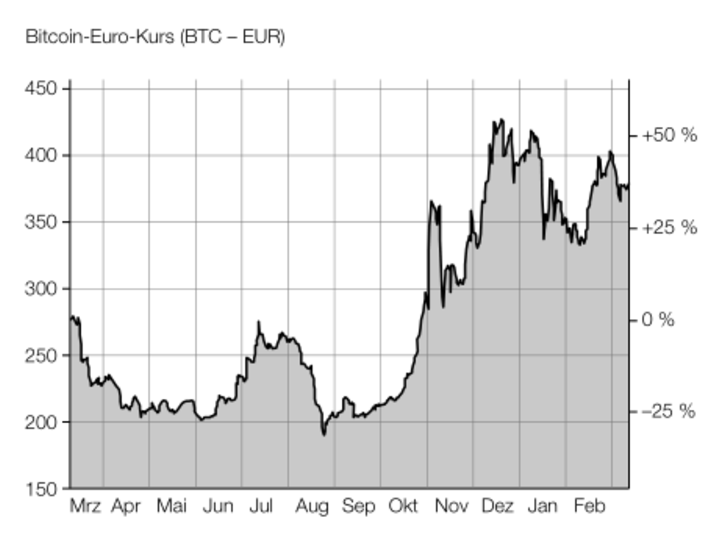
\includegraphics{../Bilder/Bild92-1.eps}}
\end{center}

\subsection{Aufgabenstellung:}
\begin{enumerate}
	\item Gib an, in welchem der Monate von April 2015 bis Dezember 2015 der Bitcoin-Euro-Kurs jeweils vom Monatsanfang bis zum Monatsende absolut am stärksten gefallen ist, und gib diesen Kursverlust in Euro an!\leer
	
	Monat:\,\antwort[\rule{3cm}{0.3pt}]{August}\leer
	
	Kursverlust:\,\antwort[\rule{3cm}{0.3pt}]{$\approx$ \EUR{55} Toleranzintervall: $[50;70]$}
	
	Es sei $K_1$ der Bitcoin-Euro-Kurs zum Beginn des betreffenden Monats, $K_2$ der Bitcoin-Euro-Kurs am Ende des betreffenden Monats sowie $AT$ die Anzahl der Tage des betreffenden Monats.
	
	Berechne den ungefähren Wert des Ausdrucks $\dfrac{K_2-K_1}{AT}$ und interpretiere das Ergebnis im gegebenen Kontext!
	
	\item Anfang Jänner 2016 waren ca. 15 Millionen Bitcoins im Umlauf. Die $t$ Jahre nach dem Jahr 2009 im Umlauf befindliche Menge an Bitcoins ist annährend $f(t)=21\cdot 10^6-21\cdot 10^6\cdot e^{-0,18\cdot t}$. Damit ist $f(0)$ die zu Anfang Jänner 2009 im Umlauf befindliche Menge an Bitcoins.
	
	Bestimmen und interpretiere die relative (prozentuelle) Änderung der im Umlauf befindlichen Menge an Bitcoins im Zeitintervall $[7;8]$!
	
	Gib eine Gleichung an, mit der derjenige Zeitpunkt berechnet werden kann, ab dem nur mehr eine Million Bitcoins in Umlauf gebracht werden kann, und ermittle diesen Zeitpunkt!
	
	\item Eine Untersuchung der Demografie von Bitcoin-Usern hat ergeben, dass weltweit 88\,\% der Bitcoin-User männlich sind.\\
Es soll festgestellt werden, wie hoch dieser Prozentsatz in Österreich ist. Dazu wird eine große Anzahl an Personen befragt. Diese Befragung ergibt, dass 171 der befragten Personen Bitcoin-User sind, und von diesen 171 Personen sind 138 männlich.

\fbox{A} Gib aufgrund dieser Daten ein symmetrischen 95-\%-Konfidenzintervall für den unbekannten Anteil der männlichen Bitcoin-User unter allen Bitcoin-Usern in Österreich an!

Gib an, welches Konfidenzniveau zur Berechnung eines solchen Intervalls mindestens angenommen werden muss, damit der weltweit ermittelte Anteil von 88\,\% in diesem Intervall enthalten ist!

	\end{enumerate}
	
	\antwort{
\begin{enumerate}
	\item \subsection{Lösungserwartung:} 

$\dfrac{K_2-K_1}{AT}\approx -1,8$

Mögliche Interpretation:\\
Im August 2015 betrug die durchschnittliche Kursänderung pro Tag ca. \EUR{-1,8}.\\
oder:\\
Im August 2015 betrug der durchschnittliche Kursverlust pro Tag ca. \EUR{1,8}.

Toleranzintervall: $[-2,3;-1,5]$ bzw. $[1,5;2,3]$

\item \subsection{Lösungserwartung:} 

$\dfrac{f(8)-f(7)}{f(7)}\approx 0,065$

Toleranzintervall: $[0,06;0,07]$

Mögliche Interpretation:\\
Die Anzahl der im Umlauf befindlichen Bitcoins nimmt im Zeitraum von Anfang Jänner 2016 bis Anfang Jänner 2017 um ca. 6,5\,\% zu.\leer

Mögliche Gleichung:\\
$f(t)=20\cdot 10^6$

Lösung der Gleichung: $t\approx 17$

Ungefähr Anfang Jänner 2026 kann nur mehr 1 Million Bitcoins in Umlauf gebracht werden.

Toleranzintervall: $[16;17]$ bzw. $[2025,2026]$
\item \subsection{Lösungserwartung:}

$n=171$, $h\approx 0,807$\\
$0,807\pm 1,96\cdot\sqrt{\frac{0,807\cdot(1-0,807)}{171}}\approx 0,807\pm 0,059 \Rightarrow [0,748;0,866]$

Toleranzintervall: unten: $[0,74;0,75]$ oben: $[0,86;0,87]$\leer

Mögliche Vorgehensweise:\\
$0,880-\frac{138}{171}\approx 0,073$

$0,073\leq z\cdot \sqrt{\frac{0,807\cdot(1-0,807)}{171}} \Rightarrow z\geq 2,418$

$2\cdot\Phi(2,418)-1\approx 0,984$

Das Konfidenzniveau muss mindestens 98,4\,\% betragen.

Toleranzintervall: $[0,98;0,99]$
\end{enumerate}}
	
	\end{langesbeispiel}